\documentclass[11pt]{article}
\usepackage[utf8]{inputenc}
\usepackage[a4paper]{geometry}
\usepackage[ruled,vlined]{algorithm2e}
\usepackage{graphicx}
\graphicspath{ {./images/} }
\usepackage{mathtools}
\DeclarePairedDelimiter{\ceil}{\lceil}{\rceil}

\title{
  Time Series Prediction with Genetic Programming\\
  \large Advanced Aspects of Nature-Inspired Search and Optimisation
}
\author{
  Sam Chatfield\\
  1559986
}
\date{25 March, 2019}

\begin{document}

\maketitle

\section{Algorithms}

The pseudo-code representing my Genetic Algorithm is given by Algorithm \ref{alg:ga}.
The functions INITIALISE, SELECT, CROSSOVER, and MUTATE are the genetic operators that I have chosen to use in my implementation and are given by Algorithms \ref{alg:init}, \ref{alg:sel}, \ref{alg:cross} and \ref{alg:mut} respectively.
One of my aims when creating the algorithm was to ensure convergence by keeping the algorithm elitist and able to jump from one solution to any other within the solution space.
By keeping the best solutions and implementing a mutation operator which replaces sub-trees of solutions with newly generated expressions, I have achieved these properties.
Hence, my algorithm will always reach the global optimal solution with a sufficiently large time budget.
In the case of the test data set used by the marking script, my algorithm is able to reach near-optimal solutions within a relatively short time budget.
My algorithm also ensures that there are no duplicate solutions within the population both in the initial creation of the population, and after applying the genetic operations in each generation.
This is represented in the pseudo-code by the set operations on the population variable.
The function $computeFitnesses$ within the code is a trivial function which uses the $trainingData$ to evaluate each expression in the population and then computes the mean squared error of this value over the whole population.
A trick that I have used within my implementation to improve its efficiency is that I store the fitness value of an individual so that it is not recomputed when required in a subsequent generation.
This is possible because of the immutable nature of my operations on individuals and means that there is very little relative overhead of keeping individuals from the previous generation and evaluating their fitnesses.

\begin{algorithm}[ht]
  \caption{Genetic Algorithm}
  \label{alg:ga}
  \DontPrintSemicolon
  \KwIn{lambda, trainingData, timeBudget, mutationTarget, mutationRate}
  \KwOut{The fittest solution found within the budgeted time}
  \Begin {
    population $\gets$ INITIALISE(lambda, maxDepth)\;\

    computeFitnesses(population, trainingData)\;
    population $\gets$ sortByFitness(population)\;\

    \While {$elapsedTime < timeBudget$} {
      (parents, nonParents) $\gets$ SELECT(population)\;
      children $\gets$ CROSSOVER(parents)\;
      mutated $\gets$ MUTATE(mutationTarget)\;\

      population $\gets$ population $\cup$ children $\cup$ mutated\;
      computeFitnesses(population, trainingData)\;
      population $\gets$ sortByFitness(population)\;
      population $\gets$ population[0, lambda-1]\;
    }\

    \Return {$population[0]$}\;
  }
\end{algorithm}

For the INITIALISE genetic operator, I actually implemented all three of the full, growth and ramped half-and-half methods which can be chosen as a parameter within my code.
Here I have outlined the ramped half-and-half method which is the default.
The function takes the ceiling of the computed $partSize$ to ensure that for any $lambda$ and $maxDepth$ at least lambda solutions will be generated.
At the end I then reduce the generated population to contain exactly $lambda$ individuals.

\begin{algorithm}[ht]
  \caption{INITIALISE (Ramped Half-and-Half)}
  \label{alg:init}
  \DontPrintSemicolon
  \KwIn{lambda, maxDepth}
  \KwOut{population}
  \Begin {
    population $\gets \emptyset$\;
    partSize $\gets \ceil[\Big]{\frac{lambda}{2(maxDepth - 1)}}$\;\

    \For {$d \gets 2$ \KwTo $maxDepth$} {
      population $\gets$ population $\cup$ fullMethod(partSize, d)\;
      population $\gets$ population $\cup$ growthMethod(partSize, d)\;
    }\

    \Return {$population[0, lambda$-$1]$}
  }
\end{algorithm}

The SELECT genetic operator I have implemented is a simple truncation selection which returns pairs of individuals chosen to be passed to CROSSOVER and also all of the solutions not chosen to be parents at all.
Using truncation selection leaves room for improvement and I believe the diversity of solutions could potentially be increased by using some kind of stochastic sort and then selecting from the result of that.
The fittest $N$ solutions could be chosen to be sorted correctly, and then the remaining solutions in the population could be sorted with some probability $P$ of sorting them out-of-order; where $N$ and $P$ would be tunable parameters.
This keeps the algorithm elitist but would allow for more exploration of the search space.

\begin{algorithm}[ht]
  \caption{SELECT (Truncation)}
  \label{alg:sel}
  \DontPrintSemicolon
  \KwIn{N, sortedPopulation}
  \KwOut{(parentPairs, nonParents)}
  \Begin {
    parents $\gets$ sortedPopulation[0, N-1]\;
    parentPairs $\gets$ zip(parents[evens], parents[odds])\;\

    nonParents $\gets$ sortedPopulation[N, end]\;\

    \Return {$(parentPairs, nonParents)$}
  }
\end{algorithm}

The CROSSOVER approach I have implemented is the Branch Swap method where nodes are chosen uniformly at random in both parent expression trees, and then the sub-trees from those nodes are swapped to create two child solutions.
My actual Python implementation does this in an immutable way so that the parent solutions are preserved in the population and the child solutions are simply added to it.

\begin{algorithm}[ht]
  \caption{CROSSOVER (Branch Swap)}
  \label{alg:cross}
  \DontPrintSemicolon
  \KwIn{parentPairs}
  \KwOut{children}
  \Begin {
    children $\gets \emptyset$\;\

    \For {(p1, p2) $\in$ parentPairs} {
      p1Idx $\gets$ rand(0, length(p1))\;
      p2Idx $\gets$ rand(0, length(p2))\;\

      p1Subtree $\gets$ subtreeAt(p1, p1Idx)\;
      p2Subtree $\gets$ subtreeAt(p2, p2Idx)\;\

      c1 $\gets$ replaceSubtreeAt(p1, p1Idx, p2Subtree)\;
      c2 $\gets$ replaceSubtreeAt(p2, p2Idx, p1Subtree)\;\

      children $\gets$ children $\cup$ \{c1, c2\}\;
    }\

    \Return {$children$}
  }
\end{algorithm}

For the MUTATION operator, I have implemented a Branch Replacement algorithm.
Here, I choose a node in the parent uniformly at random and replace the subtree from that node with a new expression tree generated using the growth initialisation method.
Similarly to the CROSSOVER operator, my implementation performs this immutably such that at the end both the parent and child are in the population.
There is also a mutation rate parameter which gives the probability that a given mutation candidate individual will be mutated.
I also have a tunable parameter which specifies the target of mutation.
This can take the values $children$, $non\_parents$ or $children\_and\_non\_parents$ and defines whether the children generated by crossover, the non-parents from selection or both should be mutated and added to the population.

\begin{algorithm}[ht]
  \caption{MUTATE (Branch Replacement)}
  \label{alg:mut}
  \DontPrintSemicolon
  \KwIn{individuals, mutationRate, maxDepth}
  \KwOut{mutated}
  \Begin {
    mutated $\gets \emptyset$\;\

    \For {ind $\in$ individuals} {
      \If {rand(0.0, 1.0) $<$ mutationRate} {
        replIdx $\gets$ rand(length(ind))\;
        newExpr $\gets$ growthMethod(1, maxDepth)\;\

        newInd $\gets$ replaceSubtreeAt(ind, replIdx, newExpr)\;\

        mutated $\gets$ mutated $\cup$ \{newInd\}
      }
    }\

    \Return {$mutated$}
  }
\end{algorithm}

\section{Parameters}

During the creation of my genetic algorithm, I tried to parameterise as many of the algorithm design choices as possible so that experiments could be carried out later to determine an optimal combination.
In this section I will explore a few of these parameters in an attempt to optimise the genetic algorithm's performance against the test dataset utilised by the Docker marking container.

Throughout my experiments I will keep the time budget fixed to 20 seconds - one of the values used by the marking script.
My justification for this is that 20 seconds should be a reasonable amount of time for the effects of different parameter values to become noticeable; while also not being too long such that each leads to similar fitness values as a result of the convergent nature of my algorithm.
For each parameter value being tested I will use 100 independent runs and create box plots of the best fitness value returned from each run.

The first parameter that I will explore is the maximum tree depth used to initialise the population.
As part of my solution, I have implemented the full, growth and ramped half-and-half initialisation methods and all of these require a depth or maximum depth parameter.
The default method used by my solution is ramped half-and-half, so I will keep this method fixed across the experiments to determine an optimal maximum tree depth.
Box plots for the experimental results are shown in Figure \ref{fig:max_depth}.
From these results it is clear that maximum tree depths of 2, 3 and 4 are significantly better than 5 and 6 when run with a fixed time budget.
I believe this is due to the smaller tree sizes leading to faster generations and thus more generations being completed within the time budget.
This allows some of the solutions within the population to make more progress towards converging on an optimal solution.

\begin{figure}[ht]
  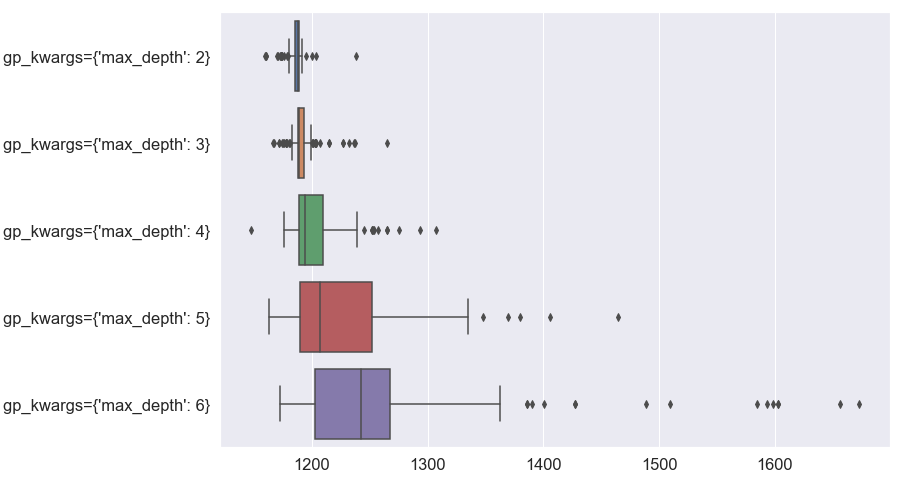
\includegraphics[scale=0.45]{max_depth}
  \centering
  \caption{Maximum tree depth experiments over the range of values $maxDepth \in [2..6]$}
  \label{fig:max_depth}
\end{figure}

The next parameters that I will run experiments for are the mutation parameters.
To begin with I will test whether it is preferable to run the mutation on just the non-parent solutions from selection or also on the child solutions from mutation.
Box plots for the results of this experiment are shown in Figure \ref{fig:mutation_target}.
Based on these results we can see that it is slightly better to mutate only the selection non-parents.
This makes intuitive sense because it means that we have to run less fitness function evaluations, leading to more generations being completed within the time budget.
Also, the children that we could mutate have already added some diversity to the population because they are a combination of two of the previous best individuals.

\begin{figure}[ht]
  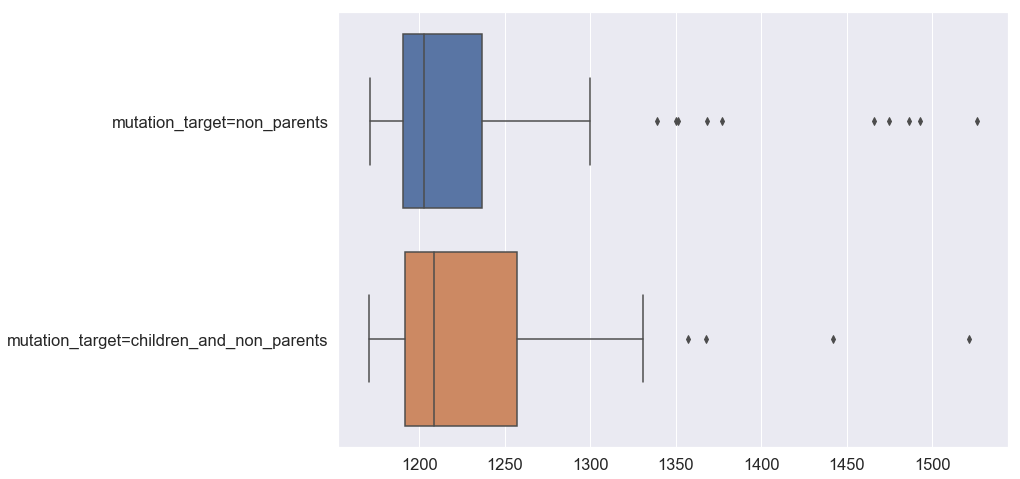
\includegraphics[scale=0.4]{mutation_target}
  \centering
  \caption{Mutation target experiments where $mutationTarget$ is either $'non\_parents'$ or $'children\_and\_non\_parents'$}
  \label{fig:mutation_target}
\end{figure}

The next parameter to test is the mutation rate.
In the context of my algorithm this means the probability that each individual in the mutation target individuals will be mutated using a branch replacement method.
The results of this are shown in Figure \ref{fig:mutation_rate} and they show that, again, the value which leads to faster generations and thus more generations gives the best results, so the best mutation rate is $0.2$.

\begin{figure}[ht]
  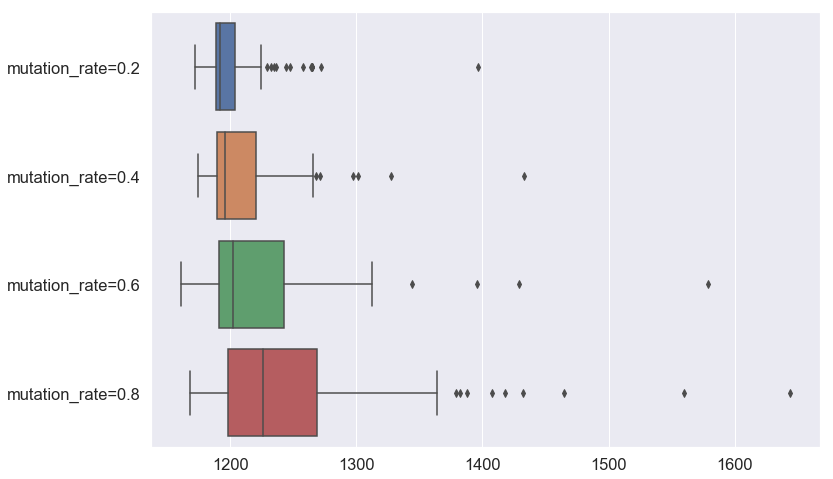
\includegraphics[scale=0.5]{mutation_rate}
  \centering
  \caption{Mutation rate experiments where $mutationRate \in \{0.2, 0.4, 0.6, 0.8\}$}
  \label{fig:mutation_rate}
\end{figure}

The final parameter that I will test is the population size denoted by lambda.
I chose to test the values in the range 40-120 in intervals of 20, this was because a reasonable population size that I had been using during the development and testing of my algorithm was 100 and so I wanted to see the effects of reducing this but also have one value higher.
The results are shown in Figure \ref{fig:lambda} and are slightly more interesting this time.
The lambda parameter essentially amounts to a trade-off between the runtime of a generation and the diversity of individuals within each generation.
The experimental results seem to show that these two factors balance each other out to some extent with the median and lower quartile of the run fitnesses being very close.
However, it seems that a value around $80$ may be preferable as the range of different fitnesses given over all the runs is lowest and most of the outlier fitnesses are closer to the median than for other values of lambda.

\begin{figure}[ht]
  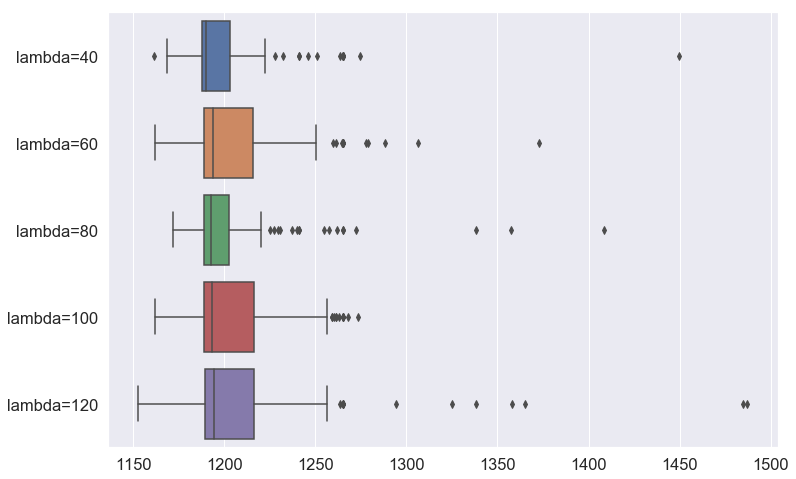
\includegraphics[scale=0.5]{lambda}
  \centering
  \caption{Population size (lambda) experiments where $lambda \in \{40, 60, 80, 100, 120\}$}
  \label{fig:lambda}
\end{figure}

\end{document}
